\chapter{Automatisierte UI Tests}
	\section{Einleitung}  %\cite{ImitationGameTuring}.
		\paragraph{} Automatisiertes UI-Testing bietet zahlreiche Vorteile in der Softwareentwicklung. Einige davon sind:
		
		\begin{itemize}
			\item Automatisierte Tests haben vergleichbare Ergebnisse und sind weniger anfällig für menschliche Fehler
			\item Höhere Testabdeckungsrate der Software
			\item Erhöhte Testabdeckung fördert debugging
			\item Erstellter Testcode kann wiederverwendet werden, wodurch das Testen leicht skalierbar wird
			\item Automatisierte Tests sind im Vergleich zu manuellen Tests viel schneller
			\item Sie sind Kosten- und Zeiteffizienter als manuelle Tests
		\end{itemize}		
		
		Der Global Quality Report zeigt, dass mehr als 60 \% der Unternehmen aufgrund der höheren Testabdeckung durch Testautomatisierung in der Lage sind, Fehler schneller zu erkennen. Darüber hinaus stellten 57 \% der Befragten fest, dass die Wiederverwendung von Testfällen durch den Einsatz von Automatisierung zunahm. Automatisiertes Testing gilt als de facto Standard in der Software Entwicklung \cite{capgemini2021microfocus}. 
		
		%Auch wenn automatisiertes Testing die nötigen manuellen Tests nicht vollständig ersetzen kann 
		
		Es äußerst wichtig, das richtige Gleichgewicht zwischen manuellen und automatisierten Tests zu finden. Jedes Projekt ist einzigartig, und es gilt, verschiedene Aspekte wie wirtschaftliche Machbarkeit, zeitliche Beschränkungen und die Art der durchzuführenden Tests zu berücksichtigen. Hier muss jedes Teams fundierte Entscheidungen treffen. Dieses Dokument dient als Entscheidungsgrundlage um ein Framework zu wählen, mit dem automatisierte UI Tests für Windows Qt-Anwendungen durchgeführt werden. Die Zielgruppe dieses Dokuments sind Softwareentwickler die mit dem C++ Qt Framework vertraut sind.
		
		\newpage
	\section{Anwendung}
		\paragraph{} Die Anwendung, die zum Vergleich der Frameworks verwendet wird, ist eine stark vereinfachte Version der Anlagensteuerungssoftware der Ambright GmbH.  
		
		\begin{figure}[t]		
			\centering
			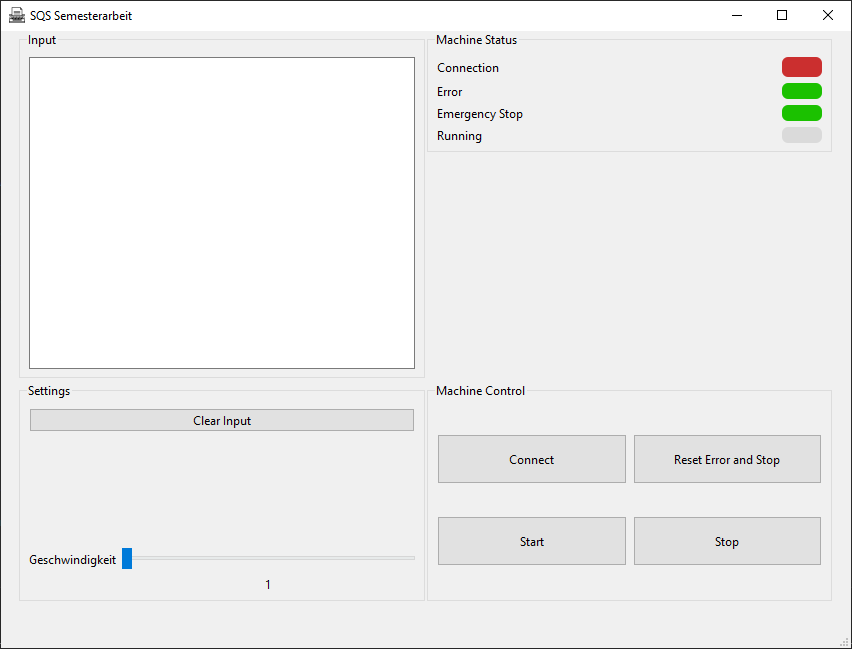
\includegraphics[width=\linewidth]{\figdir/Anwendung}
				
			\caption[Anwendung]
			{Anwendung an der die Tests Evaluiert werden}
			\label{FIG:Anwendung}
		\end{figure}
		\FloatBarrier
		
		\paragraph{} Die Anwendung lässt sich in 4 Bereiche Unterteilen. Der erste Bereich, links oben, ist ein Text Feld. Dieses Text Feld kann mit User Input gefüllt werden. Der Input wird durch drücken des Start Buttons im vierten Bereich, rechts unten, evaluiert und ausgeführt. 
		
		Im zweiten Bereich, rechts oben, sind 4 Statusanzeigen zu sehen. Die Statusanzeigen Signalisieren durch Farben den Status der Maschine. Wenn eine aktive Verbindung besteht ist die Anzeige der Connection grün, andernfalls rot. 
		Falls beim ausführen des Inputs aus dem ersten Bereich ein Fehler auftritt wird die Error Anzeige rot. Wenn kein Fehler auftritt ist sie grün eingefärbt. 
		Die Emergency Stop Anzeige zeigt an wenn der Nothalt Schalter gedrückt wurde mit roter Farbe. Falls der Nothalt Schalter nicht gedrückt wurde ist die Anzeige grün. 
		Die letzte Anzeige ist grün wenn gerade ein Script aus dem Inputfeld aufgeführt wird, andernfalls grau.
		
		Im dritten Bereich, links unten, befinden sich Settings zur Maschine. Durch den Slider kann die Geschwindigkeit innerhalb des Wertebereichs 1 - 10 eingestellt werden. Der eingestellte Geschwindigkeitswert wird durch ein Label unter dem Slider angezeigt.
		
		im letzten Bereich, rechts unten, befinden sich 4 Buttons. Der erste Button stellt eine Verbindung her. Der zweite Button setzt den Error Status zurück. Die letzten beiden Buttons sind zum Starten und Stoppen der Maschine.
		 
	\section{Anforderungen}
		\paragraph{} Die Folgende Tabelle gibt einen Überblick über die Anforderungen, welche an die UI Testing Frameworks gestellt werden. Anhand dieser Anforderungen werden die gewählten Frameworks verglichen und eine Entscheidung getroffen. Jede Anforderung ist mit einer ID versehen. Diese IDs werden im Dokument zur Referenzierung verwendet.
		%\begin{center}
					
			\begin{table}%[htdp]
				\caption{Anforderungstabelle}
				\label{TAB:Anforderungstabelle}
				\begin{tabularx}{\linewidth}{|s n g|}
				\hline
				ID & Anforderung & Metrik \\  
				\thickhline
				01 & Kosten & Kosten sollen so gering wie möglich sein \\ 
				\hline
				02 & Lizenz & Bestenfalls GPL oder vergleichbar \\
				\hline
				03 & Open Source & Source-Code öffentlich verfügbar  \\
				\hline
				04 & Integration in vorhandene Pipeline & Wie viel Zeit benötigt es die Tests in die Pipeline zu integrieren \\
				\hline
				05 & Lesbarkeit & Kann der Testcode von Entwicklern gelesen werden \\  
				\hline
				06 & Aufwand & Benötigte Zeit zum erstellen eines Tests \\
				\hline
				07 & Änderbarkeit & Benötigte Zeit zum ändern eines Tests \\
				\hline
				08 & Support / Community & Aktivität und Größe der Community (Stackoverflow, eigenes Forum, ...) \\
				\hline
				09 & Updates & Update-Zyklus des Frameworks \\
				\hline
				10 & Reife / Robustheit & Stabilität des Frameworks \\ 
				\hline
				11 & In Qt Editor ausführbar & Sind die Tests im Qt Editor ausführbar \\
				\hline 
				12 & Abdeckung der Qt Features & Mögliche Abdeckung der mit Qt erstellbaren Widgets  \\
				\hline 
				13 & Laufzeit & Wie viel Zeit beansprucht die Ausführung eines Tests \\
				\hline
				14 & Dokumentation & Umfang und Qualität der Dokumentation der Tests \\
				\hline
				15 & Auswertbarkeit der Ergebnisse & Lassen sich die Ergebnisse automatisiert auswerten \\
				\hline
			\end{tabularx}
		  \end{table}
		
		\FloatBarrier
	%	\end{center}
		
		\paragraph{} Die Kosten die für das UI Testing Framework anfallen sollen so gering wie möglich sein. Bestenfalls sollten keine Kosten anfallen. Dies ist direkt mit der Lizenz verknüpft. Eine GPL Lizenz oder vergleichbares wäre daher vorteilhaft. Wenn der Source Code des UI Testing Frameworks frei verfügbar ist bestünde die Möglichkeit, änderungen oder ergänzungen am Framework vorzunehmen, sofern die Lizenz dies erlaubt. 
		Wichtig ist, wie viel Aufwand das schreiben oder Aufnehmen eines Tests ist, sowie die Zeit die benötigt wird um mit dem Framework familär zu werden sollte gering sein. Dabei wäre es ebenso von vorteil wenn man den Testcode Lesen, nachvollziehen und verstehen kann. Ebenso wird verglichen wie viel Aufwand eine Änderung eines Tests ist, wenn sich beispielsweise die Position eines Buttons verändert. Wenn das Framework nicht in die Verwendete Pipeline integriert werden kann, kann es nicht automatisiert verwendet werden und würde damit ausgeschlossen werden. Der beste Fall hierfür wäre die Möglichkeit die Tests im Qt Editor ausführen zu können. Ein weiteres Kriterium ist die Umfangreichheit des Frameworks. Dabei wird gemessen wie weit sich alle durch Qt bereit gestellten Widgets testen lassen und ob es die Möglichkeit gibt custom Widgets zu testen. Die Laufzeit der Tests ist ebenso ein Kriterium. Wenn sich 10 Tests innerhalb von 2 Minuten ausführen und auswerten lassen. Dabei wird gleichzeitig die Anforderng der automatisierten Testauswertung in Betracht gezogen. Zuletzt wird untersucht wie groß die Community der Frameworks auf seiten wie Stackoverflow, Github oder einem eigenem Forum ist, sowie die die aussicht auf zukünftige Updates
		
		-Robustheit

%https://stackoverflow.com/questions/4163639/best-approach-to-qt-ui-testing/4166429#4166429
%https://www.ranorex.com/windows-desktop-test-automation/
%https://resources.qt.io/videos/automated-qt-gui-testing-tools-qtws21
\chapter{Open HMI Tester}
		%https://catedrasaes.org/html/projects/OHT/OHT.html
		%http://pedromateo.github.io/openhmitester/
		
		\section{Einführung Open HMI Tester}
		\paragraph{} Open HMI Tester (OHT) ist ein Framework für die Entwicklung von GUI Testing Tools. Es verwendet Echtzeit GUI Beobachtung um reale Nutzerinteraktionen aufzunehmen und abzuspielen. Dies soll Robustheit und Toleranzen für Änderungen während der Testphase bringen.
		
		OHT bietet ein plattformübergreifendes, offenes Design zur Unterstützung von ereignisbasierten GUI-Plattformen. Da es nicht in den Code eingreift kann es in laufende und ältere Entwicklungen integriert werden. Als Ergebnis bietet das Framework eine anpassbare, erweiterbare, skalierbare und robuste Basis zur Unterstützung der Automatisierung von GUI-Testprozessen.
		
		Eine fertiger Build für Windows Qt-Anwendungen wird von OHT Angeboten. Dieser Build wird in dieser Arbeit verwendet.
		
		\section{Testaufbau}
		\section{Test Beispiele}
		
\chapter{QT Test}
		%https://doc.qt.io/qt-5/qttestlib-tutorial3-example.html
		%http://blog.davidecoppola.com/2018/01/gui-unit-testing-with-qt-test-introduction/
		
		\section{Einführung QT Test}
		\section{Testaufbau}
		\section{Test Beispiele}
		
\chapter{Vergleich}

	\section{Open HMI Tester}
	\section{Qt Test}
	\section{Vergleich}

\chapter{Fazit}
%		\begin{figure}[t]		
%			\centering
%			\includegraphics[width=\linewidth]{\figdir/TuringTest1}
%			
%			\caption[Imitation Game]
%			{Grafische Darstellung des Party-Spiels \glqq Imitation Game\grqq{} (Quelle: eigene Abbildung)}
%			\label{FIG:TuringTest1}
%		\end{figure}
		%	\FloatBarrier

%		\begin{itemize}
%			\item Store
%			\item Executive Unit
%			\item Control
%		\end{itemize}
	